%!TEX root = *.tex
%%%%%%%%%%%%%%%%%%
% カウンタのリセット
\setcounter{figure}{0}
% 問題文

次の\ajRoman{1}と\ajRoman{2}について,説明を読んで問いに答えよ.


\hang{\ajRoman{1}.}
図1のように,質量$M$,長さ$L$の一様な細い棒を,
質量の無視できるひもを用いて,水平につるしてある.
棒とひもとの角度は$\theta$であり,
ひもの他端は鉛直な壁の1点に結んである.
棒と壁との間には摩擦があり,静止摩擦係数を$\mu$とする.
また,重力加速度を$g$とする.


\begin{enumerate}[(1)]
  \setlength{\leftskip}{-1zw}
  \setlength{\itemindent}{1zw}\setlength{\labelsep}{0.5zw}
  \setlength{\labelwidth}{1zw}\setlength{\leftmargin}{1zw}
  \setlength{\itemsep}{0.5\baselineskip}
  \item ひもが棒を引く力の大きさ$T$はいくらか.$M,\,L,\,\theta,\,g$のうち必要なものを用いて表せ.
  \item 棒がすべり落ちないためには,静止摩擦係数$\mu$はいくら以上でなければならないか,$M,\,L,\,\theta,\,g$のうち必要なものを用いて表せ.
\end{enumerate}

次に,棒の右端に大きさの無視できる質量$m$のおもりをかけ,
おもりの位置を徐々に左にずらしていった.


\begin{enumerate}[(1)]
  \setlength{\leftskip}{-1zw}
  \setlength{\itemindent}{1zw}\setlength{\labelsep}{0.5zw}
  \setlength{\labelwidth}{1zw}\setlength{\leftmargin}{1zw}
  \setlength{\itemsep}{0.5\baselineskip}
  \addtocounter{enumi}{2}
  \item $m=M$,$\tan{\theta}=0.75$,$\mu =0.90$の場合,おもりの位置が壁から$\alpha L$より小さくなったところで棒がすべりはじめた.
  $\alpha$の値を有効数字2桁で求めよ.
\end{enumerate}


\hang{\ajRoman{2}}
図2のように,地球の重心を中心として,等速円運動する質量$m$の人工衛星を考える.
地球の半径を$R$,地表での重力加速度の大きさを$g$とする.
人工衛星の地表からの高度を$h$とする.
ただし,地球は密度が一様な完全な球体で,
人工衛星の大きさは無視できるものとする.
また,地球の自転,公転,他の物体の影響,および空気抵抗は無視できる.
必要ならば$\sqrt{2}=1.41$を用いよ.


\begin{enumerate}[(1)]
  \setlength{\leftskip}{-1zw}
  \setlength{\itemindent}{1zw}\setlength{\labelsep}{0.5zw}
  \setlength{\labelwidth}{1zw}\setlength{\leftmargin}{1zw}
  \setlength{\itemsep}{0.5\baselineskip}
  \addtocounter{enumi}{3}
  \item 人工衛星にはたらく万有引力の大きさと,無限遠点を基準点としたときの万有引力による位置エネルギーを,$m,\,R,\,g,\,h$のうち必要なものを用いて表せ.
  \item 人工衛星の速さを$m,\,R,\,g,\,h$のうち必要なものを用いて表せ.
  また,人工衛星が地表すれすれ$(h=0\,\text{m})$を飛ぶ場合の速さの値を有効数字2桁で求めよ.
  ただし,$R=6.4\times 10^6\,\text{m},\,g=9.8\,\text{m}/\text{s}^2$とする.
  \item 地表すれすれを飛ぶ人工衛星に,力学的エネルギーを与えて,高度$h=2R$の円軌道に移すことを考える.このとき,人工衛星に与えるべき最小のエネルギーを,$m,\,R,\,g$のうち必要なものを用いて表せ.
\end{enumerate}

\begin{figure}[H]
  \centering
  \begin{minipage}[b]{.3\columnwidth}
    \centering
    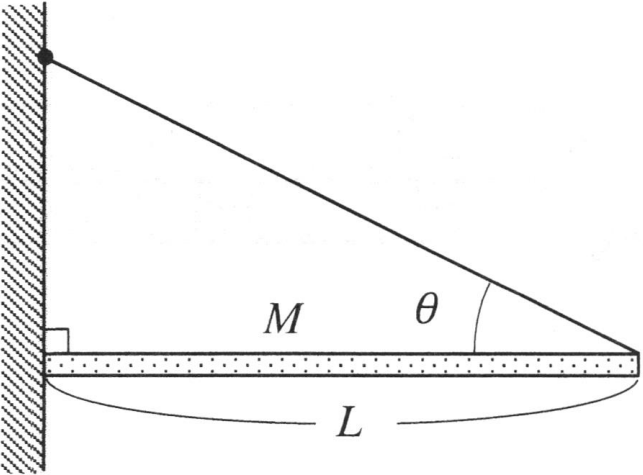
\includegraphics[width=\columnwidth]{../graphs/hamamatsu_23_2-1.png}
    \caption{}
  \end{minipage}
  \hspace{.1\columnwidth}
  \begin{minipage}[b]{.3\columnwidth}
    \centering
    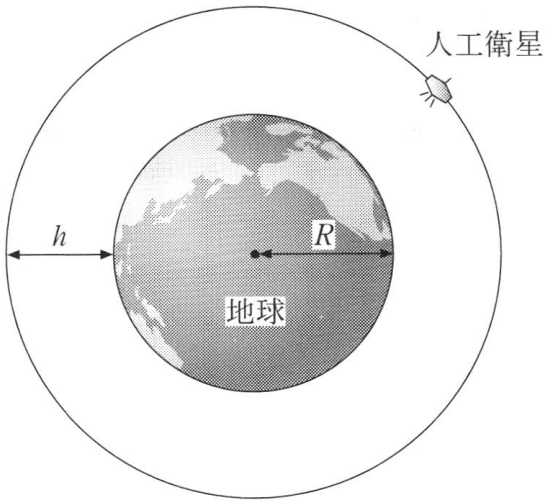
\includegraphics[width=\columnwidth]{../graphs/hamamatsu_23_2-2.png}
    \caption{}
  \end{minipage}
\end{figure}



% メモ
\begin{comment}

\end{comment}


%%%%%%%%%%%%%%%%%%
